\documentclass[xcolor=pdftex,dvipsnames,table]{beamer}
\mode<presentation>
\usetheme{boxes}
\setbeamertemplate{navigation symbols}{}
% http://www.latex-community.org/forum/viewtopic.php?f=4&t=6694
\setbeamertemplate{navigation symbols}{\raisebox{5pt}{\makebox[\paperwidth]{\hfill\makebox[10pt]{\scriptsize\insertframenumber\vspace{1ex}}}}}
\setbeamertemplate{footline}[frame number]
\setbeamertemplate{blocks}[shadow=false]
\setbeamercolor*{block title}{fg=structure,bg=RoyalBlue!10}
\setbeamercolor*{block title example}{fg=BrickRed,bg=Goldenrod!10}
\setbeamercolor*{block title alerted}{fg=white,bg=black}
\addtobeamertemplate{block begin}{\pgfsetfillopacity{0.8}}{\pgfsetfillopacity{1}}
\rowcolors{1}{RoyalBlue!20}{RoyalBlue!5}

%\DeclareGraphicsRule{*}{mps}{*}{}

\usepackage{latexsym}
\usepackage{hyperref}

\raggedright

\newcount\lecturecount
\lecturecount=0
\AtBeginLecture{%
    \advance\lecturecount by 1
    \date{}
    \begin{frame}
    \begin{center}
    \titlepage
    \ifnum\lecturecount=1
    Part \the\lecturecount: \insertlecture
    \else
    Part \the\lecturecount: \insertlecture
    \fi
    \end{center}
    \end{frame}
}

\begin{document}


\title{\color{blue}Natural Language Processing}

\author{Anoop Sarkar \\ {\tt http://anoopsarkar.github.io/nlp-class}}
\institute{}
%\date{}
     
{
\setbeamertemplate{navigation symbols}{}
\addtocounter{framenumber}{-1}
\begin{frame}
\begin{center}
\vspace{1cm}
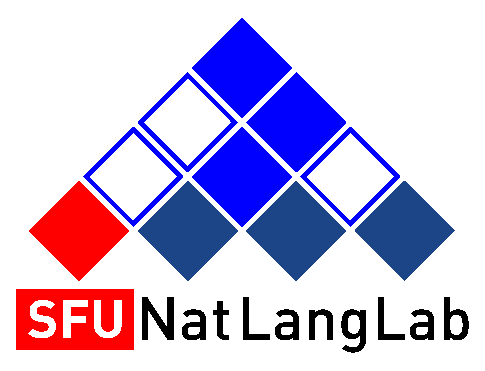
\includegraphics[scale=0.4]{figures/natlang-cky-logo.eps}
\end{center}
\titlepage
\end{frame}
}



\lecture{Machine Translation}{}

\section{Introduction to Machine Translation}
\frame{\tableofcontents[currentsection]}

\begin{frame}
\frametitle{Basic Terminology}
\begin{block}{Translation}
We will consider translation of 
\begin{itemize}
\item a source language string in French, called \textbf{f} 
\item into a target language string in English, called \textbf{e}.
\end{itemize}
\end{block}\pause
\begin{block}{\textit{A priori} probability: $\Pr(\textbf{e})$}
The chance that \textbf{e} is a valid English string.\\
What is better? $\Pr(\textit{I like snakes})$ or $\Pr(\textit{snakes like I})$
\end{block}\pause
\begin{block}{Conditional probability: $\Pr(\textbf{f} \mid \textbf{e})$}
The chance of French string \textbf{f} given \textbf{e}. \\
What is the chance of French string \textit{maison bleue} given the English string \textit{I like snakes}?
\end{block}
\end{frame}

\begin{frame}
\frametitle{Basic Terminology}
\begin{block}{Joint probability: $\Pr(\textbf{e}, \textbf{f})$}
The chance of both English string \textbf{e} and French string \textbf{f} occuring together.
\begin{itemize}[<+->]
\item If \textbf{e} and \textbf{f} are independent (do not influence each other) then 
\[ \Pr(\textbf{e}, \textbf{f}) = \Pr(\textbf{e}) \Pr(\textbf{f}) \]
\item If \textbf{e} and \textbf{f} are not independent (they do influence each other) then
\[ \Pr(\textbf{e}, \textbf{f}) = \Pr(\textbf{e}) \Pr(\textbf{f} \mid \textbf{e}) \]
\end{itemize}\pause
Which one should we use for machine translation?
\end{block}
\end{frame}

\begin{frame}
\frametitle{Machine Translation}
\begin{block}{}
Given French string \textbf{f} find the English string \textbf{e} that maximizes $\Pr(\textbf{e} \mid \textbf{f})$
\[ \textbf{e}^\ast = \arg\max_{\textbf{e}} \Pr(\textbf{e} \mid \textbf{f}) \]
This finds the \textit{most likely} translation $\textbf{e}^\ast$
\end{block}
\end{frame}

\begin{frame}
\def\blockdist{2.0}
\begin{alertblock}{Alignment Task}
\begin{tikzpicture}[node distance=2.5cm,auto,>=latex']
    \node (a) {Program};
    \path (a.140)+(-\blockdist,0) node (b) {\textbf{e}};
    \path (a.-140)+(-\blockdist,0) node (c) {\textbf{f}};
    \node (d) [right of=a] {$\Pr(\textbf{e} \mid \textbf{f})$};
    \path[->] (b) edge (a);
    \path[->] (c) edge (a);
    \path[->] (a) edge (d);
\end{tikzpicture}
\end{alertblock}
\begin{alertblock}{Translation Task}
\begin{tikzpicture}[node distance=2.5cm,auto,>=latex']
    \node (a) {Program};
    \node (b) [left of=a] {\textbf{f}};
    \path (a.140)+(3.0,1) node (c) {$\textbf{e}_1: \Pr(\textbf{e}_1 \mid \textbf{f})$};
    \path (a.-140)+(3.0,-1) node (d) {$\textbf{e}_n: \Pr(\textbf{e}_n \mid \textbf{f})$};
    \path (3.0,0) node (e) {$\vdots$};
    \path[->] (b) edge (a);
    \path[->] (a) edge (c);
    \path[->] (a) edge (d);
\end{tikzpicture}
\end{alertblock}
\end{frame}

\begin{frame}
\frametitle{Bayes' Rule}
\begin{block}{Bayes' Rule}
\[ \Pr( \textbf{e} \mid \textbf{f} ) = \frac{ \Pr(\textbf{e}) \Pr(\textbf{f} \mid \textbf{e}) }{ \Pr(\textbf{f}) } \]
\end{block}\pause
\begin{block}{Exercise}
Show the above equation using the definition of $P(\textbf{e}, \textbf{f})$ and the chain rule.
\end{block}
\end{frame}

\begin{frame}
\frametitle{Noisy Channel Model}
\begin{block}{Use Bayes' Rule}
\begin{eqnarray*}
\textbf{e}^\ast & = & \arg\max_{\textbf{e}} \Pr(\textbf{e} \mid \textbf{f}) \\
& = & \arg\max_{\textbf{e}} \frac{ \Pr(\textbf{e}) \Pr(\textbf{f} \mid \textbf{e}) }{ \Pr(\textbf{f}) } \\
& = & \arg\max_{\textbf{e}} \Pr(\textbf{e}) \Pr(\textbf{f} \mid \textbf{e})
\end{eqnarray*}
\end{block}\pause
\begin{block}{Noisy Channel}
\begin{itemize}
\item Imagine a French speaker has \textbf{e} in their head
\item By the time we observe it, \textbf{e} has become ``corrupted'' into \textbf{f}
\item To recover the most likely \textbf{e} we reason about 
\begin{enumerate}
\item What kinds of things are likely to be \textbf{e}
\item How does \textbf{e} get converted into \textbf{f}
\end{enumerate}
\end{itemize}
\end{block}
\end{frame}

\begin{frame}
\frametitle{Machine Translation}
\begin{block}{Noisy Channel Model}
\begin{eqnarray*}
\textbf{e}^\ast & = & \arg\max_{\textbf{e}} \underbrace{\Pr(\textbf{e})}_{\color{red}\textbf{Language Model}} \pause \cdot \underbrace{\Pr(\textbf{f} \mid \textbf{e})}_{\color{blue}\textbf{Alignment Model}}
\end{eqnarray*}
\end{block}\pause
\begin{block}{Training the components}
\begin{itemize}[<+->]
\item \color{red}\textbf{Language Model}: $n$-gram language model with smoothing. \\
Training data: lots of monolingual \textbf{e} text.
\item \color{blue}\textbf{Alignment/Translation Model}: learn a mapping between \textbf{f} and \textbf{e}. \\
Training data: lots of translation pairs between \textbf{f} and \textbf{e}.
\end{itemize}
\end{block}
\end{frame}

\begin{frame}
\frametitle{Word reordering in Translation}
\begin{block}{Candidate translations}
Every candidate translation \textbf{e} for a given \textbf{f} has two factors:
\[ \Pr( \textbf{e} ) \Pr( \textbf{f} \mid \textbf{e} ) \]
What is the contribution of $\Pr(\textbf{e})$?
\end{block}\pause
\begin{alertblock}{Exercise: Bag Generation}
Put these words in order:\\
\textit{have programming a seen never I language better}
\end{alertblock}\pause
\begin{alertblock}{Exercise: Bag Generation}
Put these words in order:\\
\textit{actual the hashing is since not collision-free usually the is less perfectly the of somewhat capacity table}
\end{alertblock}
\end{frame}

\begin{frame}
\frametitle{Word reordering in Translation}
\begin{block}{Candidate translations}
Every candidate translation \textbf{e} for a given \textbf{f} has two factors:
\[ \Pr( \textbf{e} ) \Pr( \textbf{f} \mid \textbf{e} ) \]
What is the contribution of $\Pr( \textbf{f} \mid \textbf{e} )$?
\end{block}\pause
\begin{alertblock}{Exercise: Bag Generation}
Put these words in order:\\
\textit{love John Mary}
\end{alertblock}
\begin{alertblock}{Exercise: Word Choice}
Choose between two alternatives with similar scores $\Pr( \textbf{f} \mid \textbf{e} )$:\\
\textit{she is in the end zone} \\
\textit{she is on the end zone} 
\end{alertblock}
\end{frame}

\begin{frame}
\frametitle{Machine Translation}
\begin{block}{Noisy Channel Model}
Every candidate translation \textbf{e} for a given \textbf{f} has two factors:
\[ \Pr( \textbf{e} ) \Pr( \textbf{f} \mid \textbf{e} ) \]
\end{block}\pause
\begin{block}{Translation Modeling}
\begin{itemize}[<+->]
\item $\Pr( \textbf{f} \mid \textbf{e} )$ does not need to be perfect because of the $\Pr( \textbf{e} )$ factor.
\item $\Pr( \textbf{e} )$ models \textbf{fluency}.
\item $\Pr( \textbf{f} \mid \textbf{e} )$ models the transfer of \textbf{content}.
\item This a \textit{generative model} of translation.
\end{itemize}
\end{block}
\end{frame}

\begin{frame}
\frametitle{$\Pr( \textbf{f} \mid \textbf{e} )$: How does English become French?}
\begin{alertblock}{English $\Rightarrow$ Meaning $\Rightarrow$ French}
\begin{itemize}
\item English to meaning representation: \\
\textit{John must not go} $\Rightarrow$ \textsc{obligatory(not(go(john)))} \\
\textit{John may not go} $\Rightarrow$ \textsc{not(permitted(go(john)))}
\item Meaning representation to French
\end{itemize}
\end{alertblock}\pause
\begin{alertblock}{English $\Rightarrow$ Syntax $\Rightarrow$ French}
\begin{itemize}
\item Parsed English: \\
\textit{Mary loves soccer} $\Rightarrow$ \textit{(S (NP Mary) (VP (V loves) (NP soccer)))}
\item Parse tree to French parse tree: \\
\textit{(S (NP Mary) (VP (V loves) (NP soccer)))} $\Rightarrow$ \textit{(S (NP Mary) (VP (V aime) (NP le football)))}
\end{itemize}
\end{alertblock}
\end{frame}

\begin{frame}
\frametitle{$\Pr( \textbf{f} \mid \textbf{e} )$: How does English become French?}
\begin{alertblock}{English words $\Rightarrow$ French words}
\begin{itemize}
\item Simplest model, map English words to French words
\item Corresponds to an alignment between English and French:
\[ \Pr( \textbf{f} \mid \textbf{e} ) = \Pr(f_1, \ldots, f_I, a_1, \ldots, a_I \mid e_1, \ldots, e_J) \]
\end{itemize}
\end{alertblock}
\end{frame}

\begin{frame}
\frametitle{Machine Translation}
\begin{block}{The IBM Models}
\begin{itemize}[<+->]
\item The first statistical machine translation models were developed at IBM Research (Yorktown Heights, NY) in the 1980s
\item The models were published in 1993: \\
{\small Brown et.\ al.\ The Mathematics of Statistical Machine Translation. \textit{Computational Linguistics}. 1993.} \\
{\small \url{http://aclweb.org/anthology/J/J93/J93-2003.pdf}}
\item These models are the basic SMT models, called: \\
IBM Model 1, IBM Model 2, IBM Model 3, IBM Model 4, IBM Model 5 \\
as they were called in the 1993 paper.
\item We use \textbf{e} and \textbf{f} in the equations in honor of their system which translated from French to English.\\
Trained on the Canadian Hansards (Parliament Proceedings)
%\item Twenty years later, they came together at a workshop called {\color{blue}\hyperlink{https://sites.google.com/site/20yearsofbitext/}{Twenty Years of Bitext}} \\
%Transcript: \url{http://cs.jhu.edu/~post/bitext/}
\end{itemize}
\end{block}
\end{frame}


\section*{Acknowledgements}

\begin{frame}
\centering
\begin{alertblock}{Acknowledgements}
Many slides borrowed or inspired from lecture notes by Michael Collins, Chris Dyer, Kevin Knight, Philipp Koehn, Adam Lopez, and Luke Zettlemoyer from their NLP course materials. 

\bigskip

All mistakes are my own.
\end{alertblock}
\end{frame}



\end{document}
